\documentclass{article}

\usepackage{neurips_2019_author_response}

\usepackage[utf8]{inputenc} % allow utf-8 input
\usepackage[T1]{fontenc}    % use 8-bit T1 fonts
\usepackage{hyperref}       % hyperlinks
\usepackage{url}            % simple URL typesetting
\usepackage{booktabs}       % professional-quality tables
\usepackage{amsfonts}       % blackboard math symbols
\usepackage{nicefrac}       % compact symbols for 1/2, etc.
\usepackage{microtype}      % microtypography
\usepackage{subcaption}
\usepackage{graphicx}
\def\setcaptionsubtype{}
\begin{document}
Thanks for the constructive comments made by all three reviewers.
Below is our response. The literature reference number follows the submitted paper reference list. 

\textbf{Common Response: Insufficient Experiment}
Our paper presents experimental results mainly on synthetic datasets but good results can also be achieved on other real-world hierarchical data. The evaluation result on NIPS-234 authorship dataset is presented in the table below, in comparison with BHCD [2] using three metric: true positive rate (TPR), true negative rate(TNR) and accuracy (ACC). For TPR and ACC our method achieves higher score. In addition, we run both algorithms on NIPS-Full authorship dataset (2864 vertices) and our algorithm runs 7 times faster than BHCD with 50 restarts.

{\centering
\InputIfFileExists{../experiment/nips-authorship/build/compare.tex}{}{}\par
}

\textbf{Common Response: Novelty and Contribution}
In theoretical model level, our paper proposed a new graph-based hierarchical clustering method (Definition 1)and analyze the hierarchical tree structure for some graph weight configuration(Proposition 1 and 3). In algorithmic level, our paper proposed a  succinct computing scheme (Algorithm 1) for parameterized graph cut function and prove its correctness (Proposition 2).

\textbf{Reviewer \#2:}
\textbf{Relation with other object optimization clustering method}
Correlation Clustering admits negative weight while our method does not; Dasgupta's cost is a function of tree while our objective is a function of partition of graph node sets. Our method is interpreted in a "maximizing information" way and is different from other graph-based formulation.
\textbf{Background of info-clustering} Besides the starting paragraph of Section 2, Info-Clustering is originally proposed to deal with genome clustering problem. Its objective function is an extension of Shannon's mutual information but impossible to compute in general cases. Currently, it is known that info-clustering is computable for hyper-graph structure.
\textbf{Experiment not explained} The configuration of each method used in the experiments is detailed in paper Appendix, and the experiment is reproducible from submitted code.
\textbf{Usage of Theorem} Theorem 3 is a basic theoretical result, sufficient condition for the trivial hierarchical tree structure and is used to prove Proposition 1 and 3. Theorem 3 is targeted at our formulation and does not apply to other objective function. It is possible similar results exist for other graph-based formulation. Your understanding of Theorem 4 is correct.
\textbf{Writing Issues} Fig.1 illustrates two interpretations (Top-Down and Bottom-Up) of our method. Your pointing about BHC is correct and it is our mistake.

\textbf{Reviewer \#5:}
\textbf{Evaluation metric} In Community Detection Experiment, Robinson-Foulds metric is used. This experiment is rerun using suggested dendrogram purity metric and the result is shown below. In most cases, our method performs better than BHCD. \textbf{Applying parametric flow algorithm directly} The method proposed by Gallo et al. applies on $g_{\lambda}(T)$, not on $h(\lambda)$, since $h(\lambda)$ is a function of partition. Our proposed method (Algorithm 1) follows the idea of Gallo et al. but simplifies original \textsf{pmf} for our specific problem.
This is also discussed in paper Appendix B.

\begin{subfigure}{0.33\textwidth}
	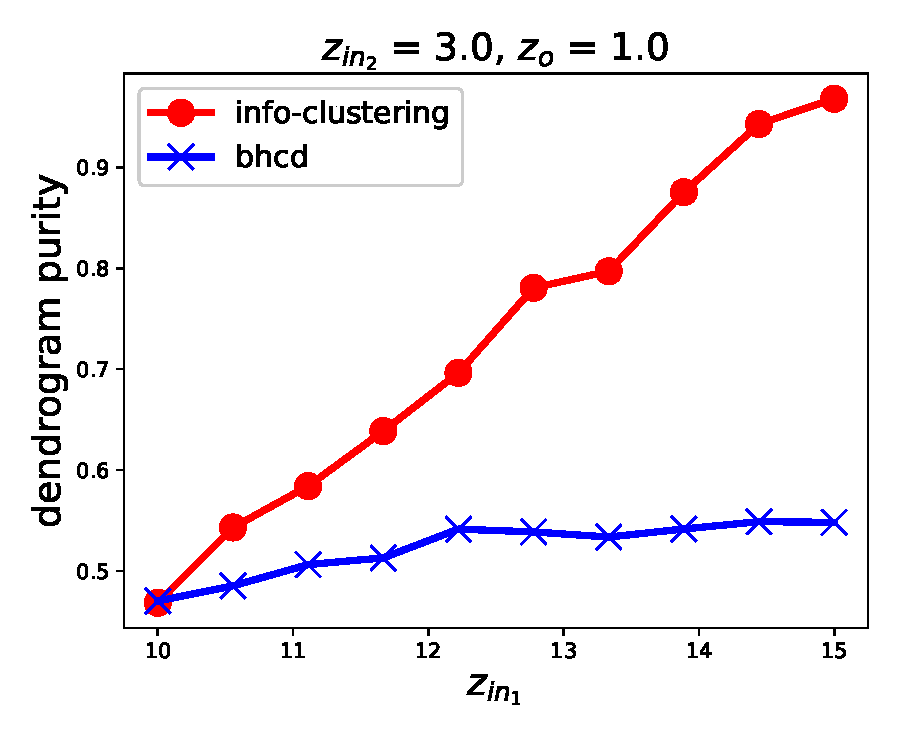
\includegraphics[width=\textwidth]{pic/z_in_1-dp.eps}
\end{subfigure}~
\begin{subfigure}{0.33\textwidth}
	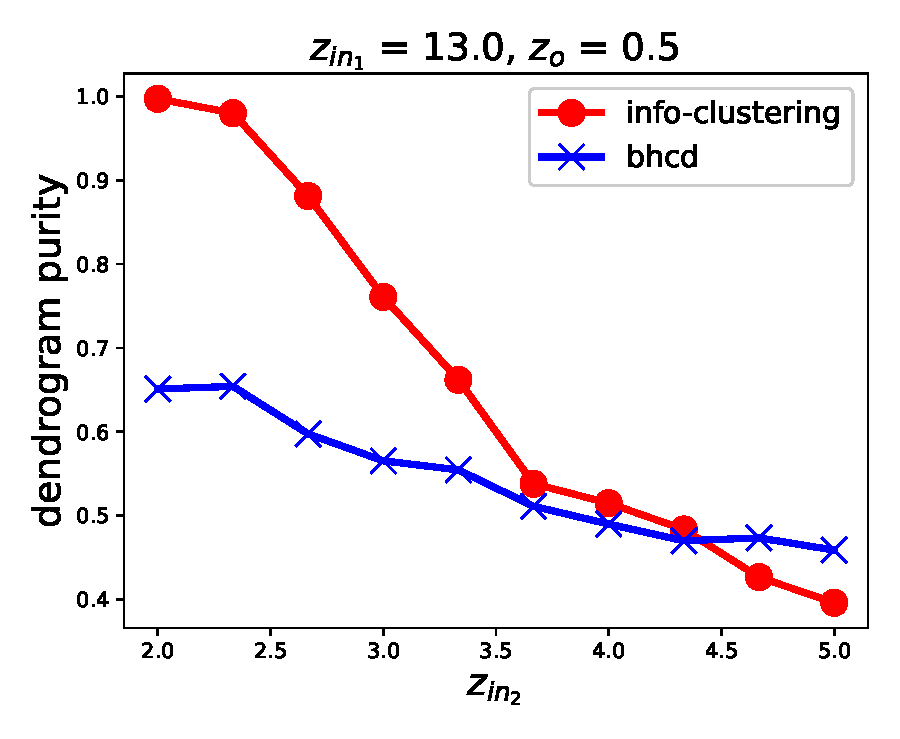
\includegraphics[width=\textwidth]{pic/z_in_2-dp.eps}
\end{subfigure}~
\begin{subfigure}{0.33\textwidth}
	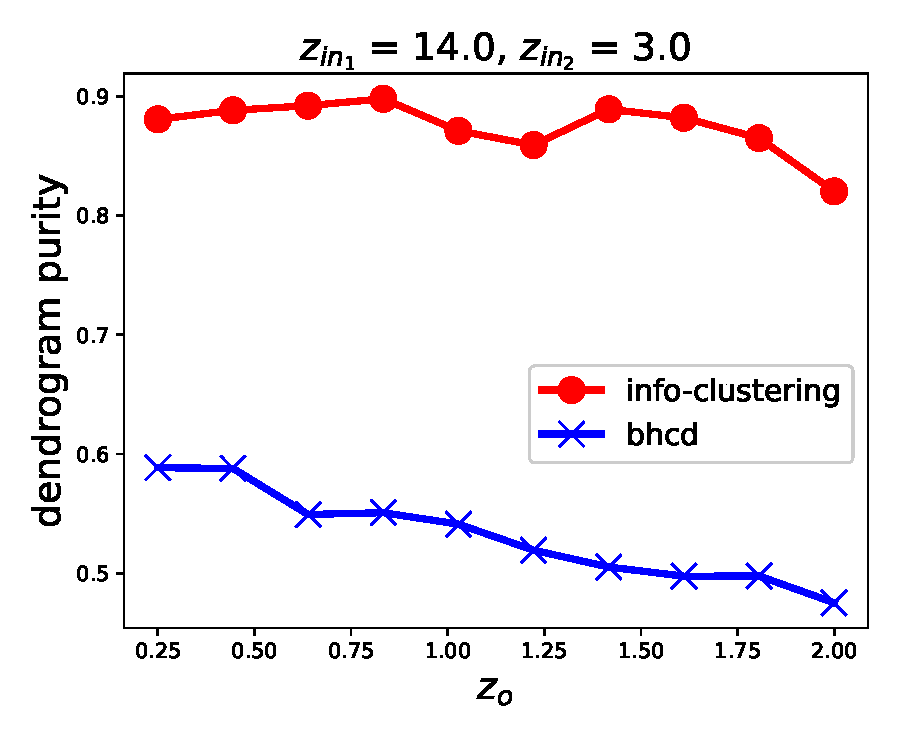
\includegraphics[width=\textwidth]{pic/z_o-dp.eps}
\end{subfigure}

\textbf{Reviewer \#3:}
\textbf{Main idea} The main idea of this paper is to use a multivariate similarity measure to do clustering task. Based on this measure, we have merging and splitting interpretation.  Merging a single pair is only one interpretation.
\textbf{Writing Issues} The function $f(\cdot)$ is defined on node set while the function $f[\cdot]$ is defined on node set partition. $f()$ is graph cut function, which means $f(\cdot)$ equals the value of graph cut. $Z_i$ represents the graph node itself while $i$ represents the node index (mentioned in footnote). Belonging should be replaced by Subset and it is our mistake. Adding the word "only" will be better.
"Information Theoretic" in the title points to the multivariate similarity measure in the paper.
\textbf{Proposition 1 Applicability} graph weight measures similarity and does not forms metric space in general. This is different to clustering method based on distance metric and we cannot deduce the limitation by this criterion.

We sincerely hope the above response can clear the doubt of all reviewers about this paper.
\end{document}
